\documentclass[main.tex]{subfiles}

\begin{document}

\tetel{1}{.33}

Ha egy vektormező valamely skalármező gradiense,
akkor annak bármely zárt görbe mentén vett integrálja
csak a kezdő- és végpontoktól függ,
vagyis független attól, hogy a kezdő- és végpontot
milyen görbével kötöttük össze.

\begin{equation*}
  \int_{\gamma} \scalar{\rvec{w}}{\differential \rvec{r}}
  = \int_a^b \scalar{\grad \left( \varphi(\rvec{r}(t)) \right)}
  {\derivative{\rvec{r}(t)}{t}} \differential t
  \overset{*}{=} \int_a^b \derivative{\varphi(\rvec{r}(t))}{t} \, \differential t
  = \varphi(\rvec{r}(b)) - \varphi(\rvec{r}(a))
\end{equation*}

\begin{equation*}
  * \hspace{5mm} \rightarrow \hspace{5mm}
  \derivative{\varphi(\rvec{r}(t))}{t}
  = \derivative{\varphi\left(
    x(t) ; \; y(t) ; \; z(t)
    \right)}{t}
  = \partialderivative{\varphi}{x} \cdot \partialderivative{x}{t}
  + \partialderivative{\varphi}{y} \cdot \partialderivative{y}{t}
  + \partialderivative{\varphi}{z} \cdot \partialderivative{z}{t}
  \hspace{10mm}
\end{equation*}


\tetel{1}{.33}

Ha $\rvec{w}$ egy olyan folytonosvektormező,
hogy a vonalmenti integrál csak a kezdő- és
végponttól függ, akkor $\exists \, \varphi$,
skalármező, hogy $\grad \, \varphi = \rvec{w}$



\jel{1}{.33}{Körintegrál}

Ha $\gamma$ zárt görbe, akkor az ő mentén vett integrált
a következőképpen szokás jelölni:
\begin{equation*}
  \oint_{\gamma} \scalar{\rvec{w}}{\differential \, \rvec{r}}
\end{equation*}



\allit{1}{.33}

Ha a görbe menti integrál értéke független az úttól,
akkor az integrál bármely zárt görbe mentén zérus.



\biz{1}{.33}

\begin{figure}[H]
  \centering
  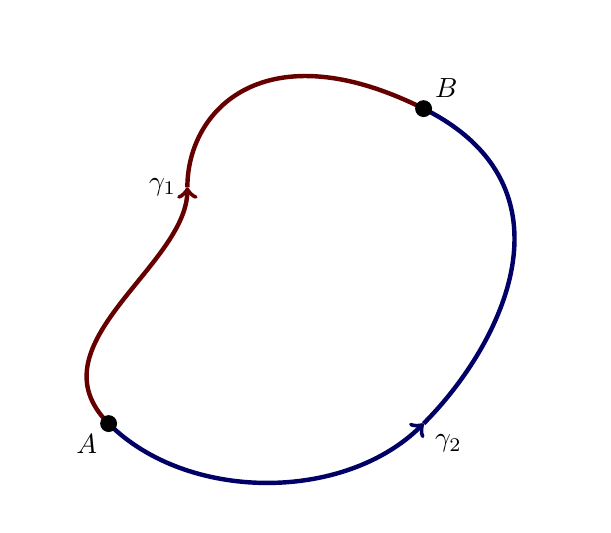
\begin{tikzpicture}
    \draw [ultra thick, ->, red!40!black ] (0,0) .. controls (-1,1) and (1,2) .. (1,3)
    node [left       , black] {$\gamma_1$};
    \draw [ultra thick    , red!40!black ] (1,3) .. controls ( 1,4) and (2,5) .. (4,4)
    node [above right, black] {$B$};

    \draw [ultra thick    , blue!40!black] (4,4) .. controls ( 6,3) and (5, 1) .. (4,0)
    node [below right, black] {$\gamma_2$};
    \draw [ultra thick, <-, blue!40!black] (4,0) .. controls (3,-1) and (1,-1) .. (0,0)
    node [below left , black] {$A$};

    \draw[fill=black] (0,0) circle (.1);
    \draw[fill=black] (4,4) circle (.1);
  \end{tikzpicture}
\end{figure}

\begin{equation*}
  \gamma = \gamma_1 \cup \gamma_2
\end{equation*}

\begin{equation*}
  \oint \limits_\gamma \scalar{\rvec{w}}{\differential \rvec{r}}
  \; =
  \int \limits_{\gamma_1} \scalar{\rvec{w}}{\differential \rvec{r}}
  + \int \limits_{-\gamma_2} \scalar{\rvec{w}}{\differential \rvec{r}}
  \; =
  \int \limits_{\gamma_1} \scalar{\rvec{w}}{\differential \rvec{r}}
  - \int \limits_{\gamma_2} \scalar{\rvec{w}}{\differential \rvec{r}}
  \; =
  0
\end{equation*}

\begin{minipage}[c]{\textwidth}
  \defi{1}{.33}{Skalármező görbe menti, ívhossz szerinti integrálja}

  \begin{minipage}[c]{.44\textwidth}
    \begin{figure}[H]
      \centering
      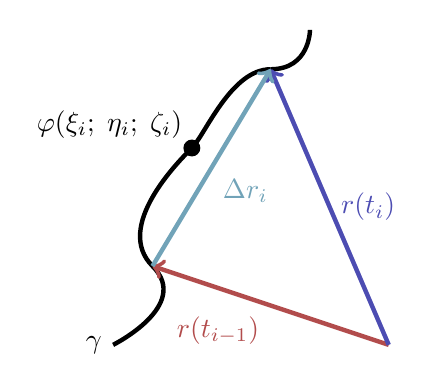
\begin{tikzpicture}
        \draw [ultra thick] (-0.5,-1) node [left] {$\gamma$} .. controls (-0.5,-1) and (0.5,-0.5) .. (0,0);
        \draw [ultra thick] (0,0) .. controls (-0.5,0.5) and (0.33,1.33) .. (0.5,1.5);
        \draw [ultra thick] (0.5,1.5) .. controls (0.67,1.67) and (1,2.5) .. (1.5,2.5);
        \draw [ultra thick] (1.5,2.5) .. controls (2,2.5) and (2,3) .. (2,3);

        \draw [ultra thick, ->, red!40!gray]
        (3,-1) -- (0,0)
        node [midway, below left] {$\rvec{r}(t_{i-1})$};

        \draw [ultra thick, ->, blue!40!gray]
        (3,-1) -- (1.5,2.5)
        node [midway, right] {$\rvec{r}(t_{i})$};

        \draw [ultra thick, ->, cyan!40!gray]
        (0,0) -- (1.5,2.5)
        node [midway, below right] {$\Delta\rvec{r}_i$};

        \draw[fill=black] (0.5,1.5) node [above left] {
          $\varphi(\xi_i ;\; \eta_i ;\; \zeta_i)$
        } circle (.1);
      \end{tikzpicture}
    \end{figure}
  \end{minipage}
  \begin{minipage}[c]{.55\textwidth}
    \begin{equation*}
      \varphi: \mathbb{R}^3 \rightarrow \mathbb{R}
      \quad
      \rvec{r}: \mathbb{R} \rightarrow \mathbb{R}^3
    \end{equation*}

    Finomítsuk a végtelenségig a
    \begin{equation*}
      \sum_i
      \varphi(\xi_i ;\; \eta_i ;\; \zeta_i)
      \norma{\Delta \rvec{r}_i}
    \end{equation*}

    összeget. Így a következő integrált kapjuk:

    \begin{equation*}
      \int \limits_\gamma
      \varphi(\xi_i ;\; \eta_i ;\; \zeta_i)
      \, \differential s.
    \end{equation*}
  \end{minipage}
\end{minipage}



\pelda{1}{20}{Súlypont számítása}



\defi{1}{.33}{Skalármező vektorértékű vonalintegrálja}

\begin{equation*}
  \int \varphi(\rvec{r}) \, \differential \rvec{r} =
  \begin{bmatrix}
    \int \varphi(\rvec{r}) \, \differential x \\
    \int \varphi(\rvec{r}) \, \differential y \\
    \int \varphi(\rvec{r}) \, \differential z \\
  \end{bmatrix}
\end{equation*}



\defi{1}{.33}{Vektormező vektorértékű vonalintegrálja}

\begin{minipage}[c]{.44\textwidth}
  \begin{figure}[H]
    \centering
    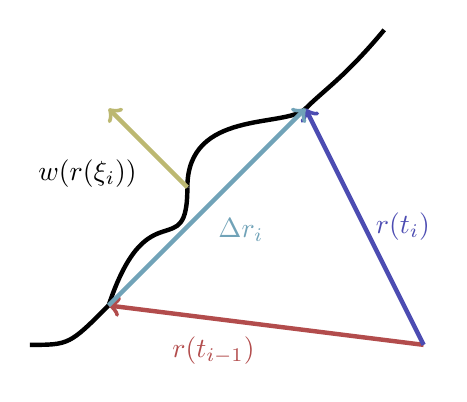
\begin{tikzpicture}
      \draw [ultra thick] (0, 0) .. controls (.5, 0) and (0.5, 0) .. (1, 0.5);
      \draw [ultra thick] (1, 0.5) .. controls (1.5, 2) and (2, 1) .. (2, 2);
      \draw [ultra thick] (2, 2) .. controls (2, 3) and (3.25, 2.75) .. (3.5, 3);
      \draw [ultra thick] (3.5, 3) .. controls (3.75, 3.25) and (4, 3.4) .. (4.5, 4);

      \draw [ultra thick, ->, red!40!gray]
      (5,0) -- (1,0.5)
      node [midway, below left] {$\rvec{r}(t_{i-1})$};

      \draw [ultra thick, ->, blue!40!gray]
      (5,0) -- (3.5,3)
      node [midway, right] {$\rvec{r}(t_{i})$};

      \draw [ultra thick, ->, cyan!40!gray]
      (1,0.5) -- (3.5,3)
      node [midway, below right] {$\Delta\rvec{r}_i$};

      \draw [ultra thick, ->, yellow!40!gray]
      (2, 2) -- (1,3)
      node [midway, below left, black] {$\rvec{w}(\rvec{r}(\xi_i))$};
    \end{tikzpicture}
  \end{figure}
\end{minipage}
\begin{minipage}[c]{.55\textwidth}
  \begin{equation*}
    \rvec{w}: \mathbb{R}^3 \rightarrow \mathbb{R}^3
    \quad
    \rvec{r}: \mathbb{R}^3 \rightarrow \mathbb{R}^3
    \quad
    \xi \in [ \; t_{i-1} \; ; \; t_i \;]
  \end{equation*}

  Finomítsuk a végtelenségig a
  \begin{equation*}
    \sum_i
    \rvec{w}(\rvec{r}(\xi_i)) \cross \Delta\rvec{r_i}
  \end{equation*}

  összeget. Így a következő integrált kapjuk:

  \begin{equation*}
    \int \limits_\gamma
    \rvec{w}(\rvec{r}) \cross \differential \rvec{r}
    =
    \int \limits_\gamma
    \rvec{w}(\rvec{r}(t)) \cross \dot{\rvec{r}}(t) \, \differential t
  \end{equation*}
\end{minipage}

%-------------------------------------------------------------------------------
%-------------------------------- Subsection 1.5 -------------------------------
%-------------------------------------------------------------------------------
\subsection{Felületmenti integrál}

\defi{0}{.33}{Reguláris felület}

Legyen $S \subset  \mathbb{R}^3$. Azt mondjuk, hogy az $S$
reguláris felület, ha $\forall \, p \in S$ ponthoz megadható
olyan $p$-t tartalmazó $V \subset \mathbb{R}^3$ nyílt halmaz
és $\varphi: U \subset \mathbb{R}^2 \rightarrow S \cap V$
leképezés, melyre teljesülnek az alábbiak:
\begin{itemize}
  \item $\varphi$ differenciálható homeomorfizmus,

  \item $\varphi$ immerzió (derivált leképezése injektív).
\end{itemize}
Ha ezek teljesülnek, akkor $\varphi$-t parametrációnak,
$V \cap S$-t  koordinátakörnyezetnek nevezzük.


\end{document}